\begin{minipage}[t][\PosterTopRowHeight][t]{\PosterTwoWidth}\vspace{0pt}
  \begin{TicketTwoPanel}{\PosterTopRowHeight}{2}{THE USUAL COMPENSATION MAKES IT WORSE}

    \noindent\begin{minipage}[c]{272mm}\centering
      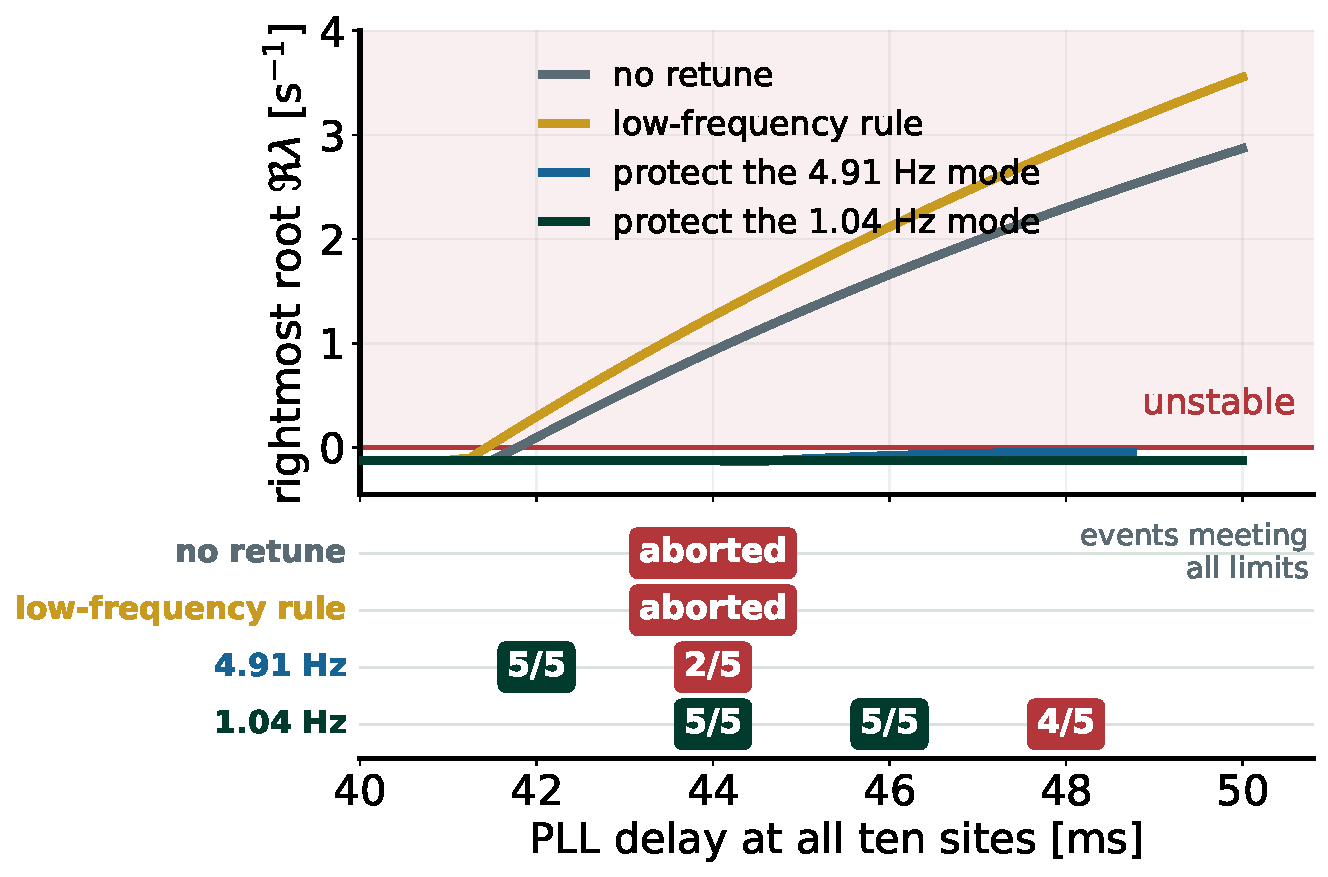
\includegraphics[width=270mm,height=190mm,keepaspectratio]{generated/figures/central.pdf}
    \end{minipage}\hfill%
    \begin{minipage}[c]{132mm}\raggedright
      {\PosterCondensed\bfseries\fontsize{74pt}{78pt}\selectfont\color{IASVermillion}12 vs 0\par}\vspace{2mm}
      {\FigureSize unstable roots at 44 ms: the low-frequency rule against protecting the 1.04 Hz mode.\par}
    \end{minipage}\par
    \vspace{2mm}
    \begin{InWords}\InWordsLabel Which mode you protect decides everything. The low-frequency rule is worse than no retune. Protecting the 1.04 Hz mode keeps the spectrum and passes 5 of 5 events.\end{InWords}

  \end{TicketTwoPanel}
\end{minipage}%
